% This is samplepaper.tex, a sample chapter demonstrating the
% LLNCS macro package for Springer Computer Science proceedings;
% Version 2.20 of 2017/10/04
%
\documentclass[runningheads]{llncs}


\usepackage{amssymb,amsmath}
% adjust the border around images
\usepackage[export]{adjustbox}
\fboxsep=5mm%padding thickness

% use this so that maths font is the same as the Keynote maths
\usepackage{stix}
%\usepackage{mathspec}
%\setmathfont(Digits,Latin,Greek)[]{}


\providecommand{\tightlist}{%
  \setlength{\itemsep}{0pt}\setlength{\parskip}{0pt}}

% This helps to correct the tilde centering in texttt  
%\usepackage{lmodern} % ruins other maths symbols
%\usepackage[T1]{fontenc}
%\usepackage{textcomp}
%\newcommand{\textapprox}{\raisebox{0.5ex}{\texttildelow}}

\usepackage{textcomp}

\makeatletter

\newcommand\midtilde@raisedtilde[1][.5]{\raisebox{#1ex}{\texttildelow}}
\def\midtilde@normaltilde{\texttildelow}

\newcommand\midtilde%
{%
  \expandafter\in@\expandafter{\f@family}%
    {cmr,cmss,cmtt,cmm,cmsy,cmx,%
    lmr,lmss,lmtt,lmm,lmsy,lmx,%
    pxr,pxss,pxm,pxsy,pxx,%
    txr,txss,txm,txsy,txx}%
  \ifin@%
    \midtilde@raisedtilde%
  \else%
    \expandafter\in@\expandafter{\f@family}%
    {pxtt,txtt}%
    \ifin@%
      \midtilde@raisedtilde[.35]%
    \else%
      \midtilde@normaltilde%
    \fi%
  \fi%
}


\usepackage[style=authoryear-comp,]{biblatex}
\addbibresource{biblio.bib}

% R Markdown
\usepackage{color}
\usepackage{fancyvrb}
\newcommand{\VerbBar}{|}
\newcommand{\VERB}{\Verb[commandchars=\\\{\}]}
\DefineVerbatimEnvironment{Highlighting}{Verbatim}{commandchars=\\\{\}}
% Add ',fontsize=\small' for more characters per line
\usepackage{framed}
\definecolor{shadecolor}{RGB}{248,248,248}
\newenvironment{Shaded}{\begin{snugshade}}{\end{snugshade}}
\newcommand{\AlertTok}[1]{\textcolor[rgb]{0.94,0.16,0.16}{#1}}
\newcommand{\AnnotationTok}[1]{\textcolor[rgb]{0.56,0.35,0.01}{\textbf{\textit{#1}}}}
\newcommand{\AttributeTok}[1]{\textcolor[rgb]{0.77,0.63,0.00}{#1}}
\newcommand{\BaseNTok}[1]{\textcolor[rgb]{0.00,0.00,0.81}{#1}}
\newcommand{\BuiltInTok}[1]{#1}
\newcommand{\CharTok}[1]{\textcolor[rgb]{0.31,0.60,0.02}{#1}}
\newcommand{\CommentTok}[1]{\textcolor[rgb]{0.56,0.35,0.01}{\textit{#1}}}
\newcommand{\CommentVarTok}[1]{\textcolor[rgb]{0.56,0.35,0.01}{\textbf{\textit{#1}}}}
\newcommand{\ConstantTok}[1]{\textcolor[rgb]{0.00,0.00,0.00}{#1}}
\newcommand{\ControlFlowTok}[1]{\textcolor[rgb]{0.13,0.29,0.53}{\textbf{#1}}}
\newcommand{\DataTypeTok}[1]{\textcolor[rgb]{0.13,0.29,0.53}{#1}}
\newcommand{\DecValTok}[1]{\textcolor[rgb]{0.00,0.00,0.81}{#1}}
\newcommand{\DocumentationTok}[1]{\textcolor[rgb]{0.56,0.35,0.01}{\textbf{\textit{#1}}}}
\newcommand{\ErrorTok}[1]{\textcolor[rgb]{0.64,0.00,0.00}{\textbf{#1}}}
\newcommand{\ExtensionTok}[1]{#1}
\newcommand{\FloatTok}[1]{\textcolor[rgb]{0.00,0.00,0.81}{#1}}
\newcommand{\FunctionTok}[1]{\textcolor[rgb]{0.00,0.00,0.00}{#1}}
\newcommand{\ImportTok}[1]{#1}
\newcommand{\InformationTok}[1]{\textcolor[rgb]{0.56,0.35,0.01}{\textbf{\textit{#1}}}}
\newcommand{\KeywordTok}[1]{\textcolor[rgb]{0.13,0.29,0.53}{\textbf{#1}}}
\newcommand{\NormalTok}[1]{#1}
\newcommand{\OperatorTok}[1]{\textcolor[rgb]{0.81,0.36,0.00}{\textbf{#1}}}
\newcommand{\OtherTok}[1]{\textcolor[rgb]{0.56,0.35,0.01}{#1}}
\newcommand{\PreprocessorTok}[1]{\textcolor[rgb]{0.56,0.35,0.01}{\textit{#1}}}
\newcommand{\RegionMarkerTok}[1]{#1}
\newcommand{\SpecialCharTok}[1]{\textcolor[rgb]{0.00,0.00,0.00}{#1}}
\newcommand{\SpecialStringTok}[1]{\textcolor[rgb]{0.31,0.60,0.02}{#1}}
\newcommand{\StringTok}[1]{\textcolor[rgb]{0.31,0.60,0.02}{#1}}
\newcommand{\VariableTok}[1]{\textcolor[rgb]{0.00,0.00,0.00}{#1}}
\newcommand{\VerbatimStringTok}[1]{\textcolor[rgb]{0.31,0.60,0.02}{#1}}
\newcommand{\WarningTok}[1]{\textcolor[rgb]{0.56,0.35,0.01}{\textbf{\textit{#1}}}}

%
\usepackage{graphicx}
% Used for displaying a sample figure. If possible, figure files should
% be included in EPS format.
%
% If you use the hyperref package, please uncomment the following line
% to display URLs in blue roman font according to Springer's eBook style:
% \renewcommand\UrlFont{\color{blue}\rmfamily}

%
\title{Symbolic Formulae for Linear Mixed Models\thanks{Supported by R Consortium}}
%
%\titlerunning{Abbreviated paper title}
% If the paper title is too long for the running head, you can set
% an abbreviated paper title here
%
\author{Emi Tanaka\inst{1} \and Francis K. C. Hui\inst{2}}
%
\authorrunning{E. Tanaka et al.}

% First names are abbreviated in the running head.
% If there are more than two authors, 'et al.' is used.
%
\institute{The University of Sydney, Camperdown NSW 2008, Australia\\\email{\href{mailto:dr.emi.tanaka@gmail.com}{\nolinkurl{dr.emi.tanaka@gmail.com}}}\\ \and Australian National University, Acton ACT 2601, Australia\\\email{\href{mailto:francis.hui@anu.edu.au}{\nolinkurl{francis.hui@anu.edu.au}}}\\}

\usepackage[unicode=true]{hyperref}
\hypersetup{
            pdftitle={Symbolic Formulae for Linear Mixed Models},
            pdfborder={0 0 0},
            breaklinks=true}

\begin{document}

%
\maketitle              % typeset the header of the contribution
%
\begin{abstract}
A statistical model is a mathematical representation of often a simplified or idealised data-generating process. A particular type of statistical model that is widely used is linear mixed models (LMMs), also called multi-level, nested, hierarchical or panel data models. LMMs are used widely in a variety of disciplines, e.g.~agriculture, ecology, econometrics, psychology and so on, owing to its flexbility of accounting for complex correlated strucures in data. This flexibility, however, have given rise to a number of ways to specify the LMMs in order to fit it via an application software. In this paper, we review the software design of LMM (and its special case, the linear models) specification, in particular with the use of symbolic model formulae, with focus on the LMM specification in popular but contrasting \texttt{lme4} and \texttt{asreml} R-packages.
%The abstract should briefly summarize the contents of the paper in
%15--250 words.
\keywords{multi-level model \and hierarchical model \and panel data model \and model specification \and model formulae \and model API \and fixed effects \and random effects}
\end{abstract}

\hypertarget{introduction}{%
\section{Introduction}\label{introduction}}

Statistical models are mathematical formulation of often simplified real world phenomena, the use which is ubiquitous in many data analyses. These models are fitted or trained computationally, often with practitioners using some readily available application software or software package. In practice, statistical models in its mathematical (or descriptive) representation would require translation to the right input argument to fit using an application software. The design of these input arguments (called application programming interface, API) can help ease the friction in fitting the user's desired model and focus user's time on important tasks, e.g.~interpreting or using the fitted model.

While there are an abundance of application software for fitting a variety of statistical models, the API is largely inconsistent and restrictive in some fashion. For example, in linear models, the intercept may or may not be included by default; and random error is assumed to be identical and independently distributed (i.i.d) with no option to modify these assumption. These inconsistencies and restrictiveness in the API cause great friction to fit the user's desired models. Some efforts have been made in this front such as by the \texttt{parsnip} package \autocite{Kuhn2018} in the R language \autocite{R2018} to implement a tidy unified interface to many preditive modelling functions (e.g.~random forest, logistic regression, linear regressoin etc) and \texttt{scikit-learn} library \autocite{scikit-learn} for machine learning in the python language \autocite{van1995python} that provides consistent API across its modules \autocite{sklearn_api}. There is, however, little effort on consistency or discussion for the software specification of linear mixed models (LMMs).

LMMs (also called hierarchical, panel data, nested or multi-level models) are widely used across many disciplines (e.g.~ecology, psychology, agriculture, finance etc) due to their flexibility to model complex, correlated structures in the data. This flexibility is primarily achieved via the inclusion of random effects and its corresponding variance-covariance structure - it is this flexibility, however, that results in major difference in model specification between software. In R, arguably the most popular general purpose package to fit LMMs is \texttt{lme4} \autocite{Bates2015}. Total downloads from RStudio CRAN mirror from \texttt{cranlogs} \autocite{cranlog} indicate there were over 2 million downloads for \texttt{lme4} in the whole of 2018, whilst other popular mixed model packages \autocites[e.g. \texttt{nlme},][]{nlme}[\texttt{rstan},][]{rstan}[\texttt{brms},][]{brmsjss}{brmsr} in the same year have less than half a million downloads. Another general purpose linear mixed model package is \texttt{asreml} \autocite{Butler2009}, which wraps the proprietary software ASreml \autocite{Gilmour2009} into the R framework. As this package is not available on CRAN, there is no comparable download logs, although, citations of its technical document indicates popular usage. In this paper, we discuss only \texttt{lme4} and \texttt{asreml} due to its active maintainance, maturity and contrasting approaches.

Both the \texttt{lme4} and \texttt{asreml} R packages employ a symbolic model formula as part of its API to specfiy the model. Symbolic model formulae define the structural component of a statistical model in an easier and often more accessible terms for practitioners. The earlier instance of symbolic model formulae for linear models was applied in Genstat \autocite{genstat} and GLIM \autocite{GLIM} with description by \textcite{Wilkinson1973}. \textcite{Chambers1993} describe the symbolic model formulae implementation for linear models in the \texttt{S} language which remains much the same in the \texttt{R} language. While the symbolic formula of linear models generally have a consistent representation and evaluation rule as implemented in \texttt{stats::formula}, this is not the case for LMMs (and mixed models more generally). The inconsistency of symbolic formulae arises mainly in the representation of random effects, with the additional need to specify the variance-covariance structure of the random effects as well as structure of the associated model matrix that governs how the random effects are mapped to (groups of) the observational units.

In Section \ref{lm}, we briefly describe the symbolic model formula in linear models.,We then describe the symbolic model formula employed in the linear mixed model \texttt{lme4} and \texttt{asreml} R packages in Section \ref{lmm}. We follow by illustrating a number of statistical models motivated by the analysis of publicly available agricultural datasets with corresponding API for \texttt{lme4} and \texttt{asreml} in Section \ref{examples}. We conclude with summary and discussion in Section \ref{discussion}.

\hypertarget{lm}{%
\section{Symbolic Formulae for Linear Models}\label{lm}}

A special case of linear mixed models is the linear (fixed) models where the model comprises of only fixed effects and a single random term (i.e.~the error) given in a matrix notation as
\begin{equation}
\boldsymbol{y} = \mathbf{X}\boldsymbol{\beta} + \boldsymbol{e}\label{eq:lm}
\end{equation}
where \(\boldsymbol{y}\) is a \(n\)-vector of response, \(\mathbf{X}\) is the \(n\times p\) design matrix for associated \(p\)-vector of fixed effects \(\boldsymbol{\beta}\) and \(\boldsymbol{e}\) is the \(n\)-vector of random error. Typically we assume \(\boldsymbol{e} \sim N(\boldsymbol{0}, \sigma^2\mathbf{I}_n)\) although this assumption is unnecessary for fitting the model under least squares.

The software specification of linear model is largely divided into two approaches: (1) input of arrays for the response \(\boldsymbol{y}\) and design matrix for fixed effects \(\mathbf{X}\) and (2) input of symbolic model formula along with data frame that define the variables in the formula. The input of data frame may be optional if the variables are defined in the parental environment, although we do not recommend such an approach due to larger potential of error (e.g.~one variable sorted while others are not).

Symbolic model formulae is heavily used to specfiy linear models in R since its first public release in 1993, inheriting most of its characteristic from S. In R, formulae have a special class \texttt{formula} and can be used for other purposes other than model specification - this type of use is beyond the scope of this paper. The history of the \texttt{formula} class in R (and S) is considerably longer than other popular languages, e.g.~the \texttt{patsy} python library \autocite{patsy} imitating R's formula was introduced in 2011 and used in \texttt{Statsmodels} library \autocite{seabold2010statsmodels} to fit a statistical model. We will limit the discussion of symbolic model formulae to those implemented in R for the rest of the paper, however, it is important to note that the conceptual framework is not limited to R.

Symbolic model formulae makes use of the variable names defined in the environment (usually through the data frame) in the specification of linear models. The left hand side (LHS) indicate the response; the right hand side (RHS) resemble its mathematical form; and the LHS and RHS is separated by \texttt{\midtilde} which can be read as ``modelled by''. E.g. the symbolic model formula \texttt{y \midtilde\ 1 + x} can be thought of as vector \texttt{y} is modelled by a linear predictor consisting of an overall intercept and variable \texttt{x}.

When the variables are numerical then the connection between the formula to its regression equation is obvious - LHS is \(\boldsymbol{y}\) and RHS correspond to the columns of the design matrix \(\mathbf{X}\) in the linear model \eqref{eq:lm}. Any transformation to the variable can be parsed in the model formula and may be used later in the pipeline (e.g.~prediction in its original scale). This contrasts when the input arguments are the design matrix and the corresponding response -- now there is an extra step required by the user to transform the data before model fitting. Such manual tranformation likely results in manual back-tranformation later in the analysis pipeline. This no doubt creates extra layer of friction for the practitioner in their day-to-day analysis. Figure \ref{fig:symbolic-lm} illustrates this connection using the \texttt{trees} dataset.

\begin{figure}
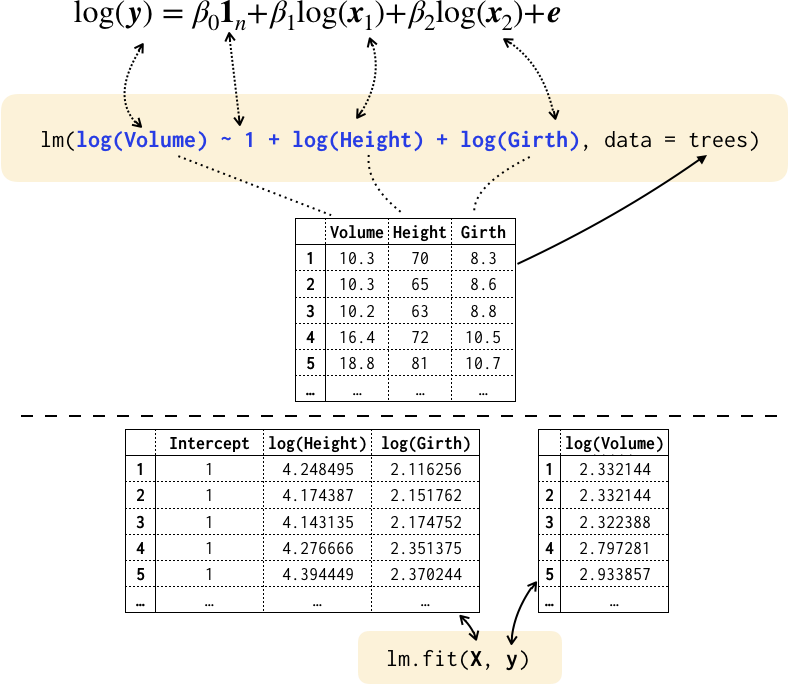
\includegraphics[width=0.9\linewidth,fbox]{images/symbolic_lm} \caption{There are two main approaches to fitting a linear model illustrated above with the fit of a linear model to the \texttt{trees} dataset: (1) top uses the \texttt{lm} function in R with input argument as a symbolic model formulae (in blue) and (2) bottom uses the \texttt{lm.fit} function in R that requires input of design matrix and the response. The latter approach is scarcely used in R, however, it is the common approach in other languages. The connection of the data column names to symbolic model formula and its resemblance to the model equation is immediately obvious. Tranformations may be automatically for later analysis for top approach (e.g.~prediction in original scale) however this likely requires manual recovery for the bottom approach. See Section \ref{trees} about the data and the model.}\label{fig:symbolic-lm}
\end{figure}



The specification of the intercept by \texttt{1} in the formula as done in Figure \ref{fig:symbolic-lm} is unnecessary in R as this is included by default. The removal of intercept is required by including \texttt{-1} or \texttt{+0} on the RHS. In this paper, the intercept is explicitly included as the resemblance to its model equation form is lost without it. While the omission of \texttt{1} is long engrained within R, we recommended to explicitly include \texttt{1} and do not recommend designing software to require explicit specification to remove intercept as currently required in R. See Section \ref{intercept} for discussion on this.

Categorical variables are typically converted to a set of dummy variables consisting of 0s and 1s indicating whether the corresponding observation belongs to the respective categorical level. For identiability, some contraint is applied, e.g.~the treatment constraint will estimate effects in comparison with a particular reference group (the default behaviour in R). In the presence of categorical variables the direct mapping of the symbolic formula to the regression equation is lost, however, the mapping is clear in converting the model equation to the so-called ANOVA model form as illustrated in Figure \ref{fig:symbolic-lm-factor} with the fit of two-way ANOVA model with interaction to the \texttt{herbicide} data.

\begin{figure}
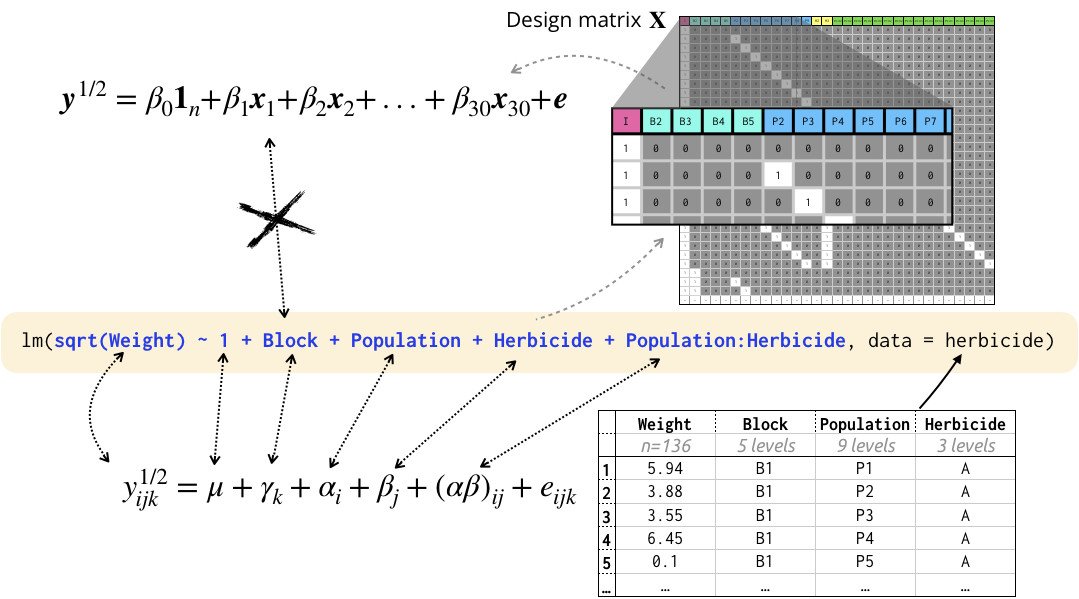
\includegraphics[width=0.9\linewidth,fbox]{images/symbolic_lm_factor} \caption{In the presence of categorical variable, the resemblance of the symbolic model formulae to its regression model form is not immediately obvious. In this case, categorical variables are transformed to a set of dummy variables with constraint applied for identifiability. As such, a single categorical variable span a number of columns in the design matrix. If the model equation is written in the form of ANOVA model (with index notation) then the categorical variables have an immediate connection to the fixed effects in the model. See \ref{grass} for more information about the data and the model.}\label{fig:symbolic-lm-factor}
\end{figure}



Interaction effects are specfied easily with symbolic model formula by use of \texttt{:} operator as seen in Figure \ref{fig:symbolic-lm-factor}. The formula in Figure \ref{fig:symbolic-lm-factor} can also be written more compactly as \texttt{sqrt(Weight)} \texttt{\midtilde\ }\texttt{1\ +\ Block\ +\ Population\ *\ Herbicide} where \texttt{*} operator fits is the short hand for main effects and the interaction effects. Further shorthand exists for her higher order interactions, e.g. \texttt{y \midtilde\ }\texttt{1\ +\ (x1\ +\ x2\ +\ x3)\^{}3} is equivalent to\\
\texttt{y \midtilde\ }\texttt{1\ +\ x1\ +\ x2\ +\ x3\ +\ x1:x2\ +\ x1:x3\ +\ x2:x3\ +\ x1:x2:x3}, a model that contains main effects, two-way and three-way interaction effects. The \texttt{1} can be included in the bracket as \texttt{y \midtilde\ }\texttt{(1\ +\ x1\ +\ x2\ +\ x3)\^{}3} to yield the same result. Perhaps surprisingly \texttt{y \midtilde\ }\texttt{(0\ +\ x1\ +\ x2\ +\ x3)\^{}3} does not include the intercept in the fitted model as \texttt{0} is converted to \texttt{-1} and carried outside the bracket and power operator. The formula simplification rule, say for \texttt{y \midtilde\ }\texttt{(0\ +\ x1\ +\ x2\ +\ x3)\^{}3}, in R can be found by

\begin{Shaded}
\begin{Highlighting}[]
\KeywordTok{formula}\NormalTok{(}\KeywordTok{terms}\NormalTok{(y }\OperatorTok{~}\StringTok{ }\NormalTok{(}\DecValTok{0} \OperatorTok{+}\StringTok{ }\NormalTok{x1 }\OperatorTok{+}\StringTok{ }\NormalTok{x2 }\OperatorTok{+}\StringTok{ }\NormalTok{x3)}\OperatorTok{^}\DecValTok{3}\NormalTok{, }\DataTypeTok{simplify =} \OtherTok{TRUE}\NormalTok{))}
\end{Highlighting}
\end{Shaded}

\begin{verbatim}
## y ~ x1 + x2 + x3 + x1:x2 + x1:x3 + x2:x3 + x1:x2:x3 - 1
## <environment: 0x7fac64b0ef28>
\end{verbatim}

\hypertarget{trees}{%
\subsection{Trees Volume: Linear Model}\label{trees}}

The \texttt{trees} data set \autocite[original data source from][built-in data in R]{minitab} contain 31 observations with 3 numerical variables. The model shown in Figure \ref{fig:symbolic-lm} is a linear model in \eqref{eq:lmm} with \(31\times 3\) design matrix \(\mathbf{X} = \begin{bmatrix}\boldsymbol{1}_{31} & \log(\boldsymbol{x}_1) & \log(\boldsymbol{x}_2)\end{bmatrix}\) where \(\boldsymbol{x}_1\) is the height of the tree and \(\boldsymbol{x}_2\) is the diameter (named \texttt{Girth} in the data) of the correponding tree; and \(\boldsymbol{y}\) is the volume of the tree.

\hypertarget{grass}{%
\subsection{Herbicide: Categorical Variable}\label{grass}}

The \texttt{herbicide} data set \autocite[original source from R. Hull, Rothamsted Research, data sourced from][]{Welham2015} contains 135 observations with 1 numerical variable (weight response) and 3 categorical variables: block, herbicide, and population of black-grass with 5, 3 and 9 levels respectively. The experiment employed has a factorial treatment structure (i.e.~27 treatments which are crosses of herbicide and population) with the complete set of treatment randomised within each of the five blocks (i.e.~it employs a randomised complete block design).

The model in Figure \ref{fig:symbolic-lm-factor} fits a linear model to the square root of the weight of the black-grass with design matrix \(\mathbf{X} = \begin{bmatrix}\boldsymbol{1}_{135} & \boldsymbol{x}_1 & \cdots & \boldsymbol{x}_{30}\end{bmatrix}\) where \(\boldsymbol{x}_1, ..., \boldsymbol{x}_4\) {[}FILL{]}. Alternatively, the model can be written as the so-called ANOVA model
\[y_{ijk} = \mu + \gamma_k + \alpha_i + \beta_j + (\alpha\beta)_{ij} + e_{ijk}\]
where index \(i\) denotes for level of population; index \(j\) for level of herbicide and indicate \(k\) for the replicate block with constraints \(\alpha_1 = \beta_1 = \gamma_1 = (\alpha\beta)_{1j}=(\alpha\beta)_{i1} = 0\). This form is equivalent with the linear regression model given in \eqref{eq:lm} when fixed effects \(\boldsymbol{\beta} = (\mu, \gamma_2,... , \gamma_5, \alpha_2, \alpha_3, ... , \alpha_9, \beta_2, \beta_3, (\alpha\beta)_{22}, (\alpha\beta)_{23}, ..., (\alpha\beta)_{93})^\top\).

\hypertarget{intercept}{%
\subsection{Specification of intercept}\label{intercept}}

\textcite{Wilkinson1973} describes many of the operators and evaluation rules with symbolic model formulae that is implemented in R (as well as other languages). These include simplification rules such as \texttt{y} \texttt{\midtilde\ }\texttt{x\ +\ x} and \texttt{y} \texttt{\midtilde\ }\texttt{x:x} to \texttt{y} \texttt{\midtilde\ }\texttt{x}. Their description however did not include about intercept. The symbolic evaluation rules governing intercept are special cases in the current implementation in R. These implementations may not be as intuitive, e.g.

\begin{itemize}
\tightlist
\item
  \texttt{y} \texttt{\midtilde\ }\texttt{1:x} simplifies to \texttt{y} \texttt{\midtilde\ }\texttt{1}, although one may expect \texttt{y} \texttt{\midtilde\ }\texttt{x};
\item
  \texttt{y} \texttt{\midtilde\ }\texttt{1*x} simplifies to \texttt{y} \texttt{\midtilde\ }\texttt{1}, which may be surprising since
\item
  \texttt{y} \texttt{\midtilde\ }\texttt{x*1} simplifies to \texttt{y} \texttt{\midtilde\ }\texttt{x}, which makes the cross operator unsymmetrial for this special case.
\end{itemize}

Some unambiguity arise from the need to explictly remove intercept, e.g.

\begin{itemize}
\tightlist
\item
  \texttt{y} \texttt{\midtilde\ }\texttt{1\ +\ (-1\ +\ x)} simplifies to \texttt{y} \texttt{\midtilde\ }\texttt{x\ -\ 1},
\item
  \texttt{y} \texttt{\midtilde\ }\texttt{-1:x} simplifies to non-sensical \texttt{y} \texttt{\midtilde\ }\texttt{1\ -\ 1}, which is equivalen to \texttt{y} \texttt{\midtilde\ }\texttt{0}.
\end{itemize}

The first point was raised by \textcite{patsy} and formula evaluation differ in \texttt{patsy} python library in this aspect. These complications arise due to explicit specification of removal of the overall intercept. Furthermore, this removes the resemblance to model equation detracting from the aim of symbolic model formula to make it accessible for practitioners.

Of course the above cases are all contrived and would rarely be used in practice.

\hypertarget{lmm}{%
\section{Linear Mixed Models}\label{lmm}}

Consider a \(n\)-vector of response \(\boldsymbol{y}\) modelled as
\begin{equation}
\boldsymbol{y} = \mathbf{X}\boldsymbol{\beta} + \mathbf{Z}\boldsymbol{b} + \boldsymbol{e}
\label{eq:lmm}
\end{equation}
where the \(\mathbf{X}\) is the design matrix for the fixed effects \(\boldsymbol{\beta}\); \(\mathbf{Z}\) is the design matrix of the random effects \(\boldsymbol{b}\) and \(\boldsymbol{e}\) is the vector of random error. We typically assume that
\[\begin{bmatrix}\boldsymbol{b}\\\boldsymbol{e}\end{bmatrix}\sim N\left(\begin{bmatrix}\boldsymbol{0}\\\boldsymbol{0}\end{bmatrix}, \begin{bmatrix}\mathbf{G} & \mathbf{0} \\ \mathbf{0} & \mathbf{R} \end{bmatrix}\right)\]
where \(\mathbf{G}\) and \(\mathbf{R}\) are the variance-covariance matrices of \(\boldsymbol{b}\) and \(\boldsymbol{e}\), respectively.

\hypertarget{lme4}{%
\subsection{\texorpdfstring{\texttt{lme4}}{lme4}}\label{lme4}}

The \texttt{lme4} R package fits a linear mixed model with the function \texttt{lmer}. The API consists of a \emph{single} formula that extends the linear model formula. More specifically, the random effects are added by surrounding the term in round brackets with grouping structure specified on the right of the vertical bar and the random terms within each group on the left of the vertical bar, e.g. \texttt{(formula\ \textbar{}\ group)}. The \texttt{formula} is evaluated under the same mechanism for symbolic model formula for linear models in Section \ref{lm} with \texttt{group} specific effects from \texttt{formula}. The \texttt{group} specific effects is assumed to be Gaussian distributed with zero mean and unstructured variance. Examples are provided in Section \ref{examples}.

\hypertarget{asreml}{%
\subsection{\texorpdfstring{\texttt{asreml}}{asreml}}\label{asreml}}

The strength of linear mixed model specification in \texttt{asreml} lies in its flexible covariance structure. The full list of covariance strucures available for \texttt{asreml} Version 3 is given in \textcite{Butler2009}. \texttt{asreml} version 4 has some slight differences as outlined in \textcite{Butler2018} although the main concept is similar: variance structures are specified with function-like terms in the model formulae, e.g. \texttt{us(factor)} will fit a \texttt{factor} effect with unstructured covariance matrix; \texttt{diag(factor)} will fit a \texttt{factor} effect with diagonal covariance matrix, i.e.~zero off-diagonal and different parameterisation in the diagonal elements. Note \texttt{factor} correspond to a categorical variable in the data. See more examples in Section \ref{examples}.

\hypertarget{examples}{%
\section{Motivating Examples}\label{examples}}

This section presents motivating examples with model specification by \texttt{lmer} or \texttt{asreml}. It should be noted that the models are not advocated to be ``correct'' but rather a plausible model that a practitioner may consider.

\hypertarget{chick}{%
\subsection{Chicken Weight: Longitudinal Analysis}\label{chick}}

The chicken weight data is originally sourced from \textcite{chickendata} and found as a built-in data set in R. It consists of the weights of 50 chickens tracked over regular time intervals (not all weights at each time points are observed). Each chicken are fed one of the 4 diets. A possible model that a user may fit to this chicken weight data is illustrated in Figure \ref{fig:symbolic-lmm} and elaborated next.

\begin{figure}
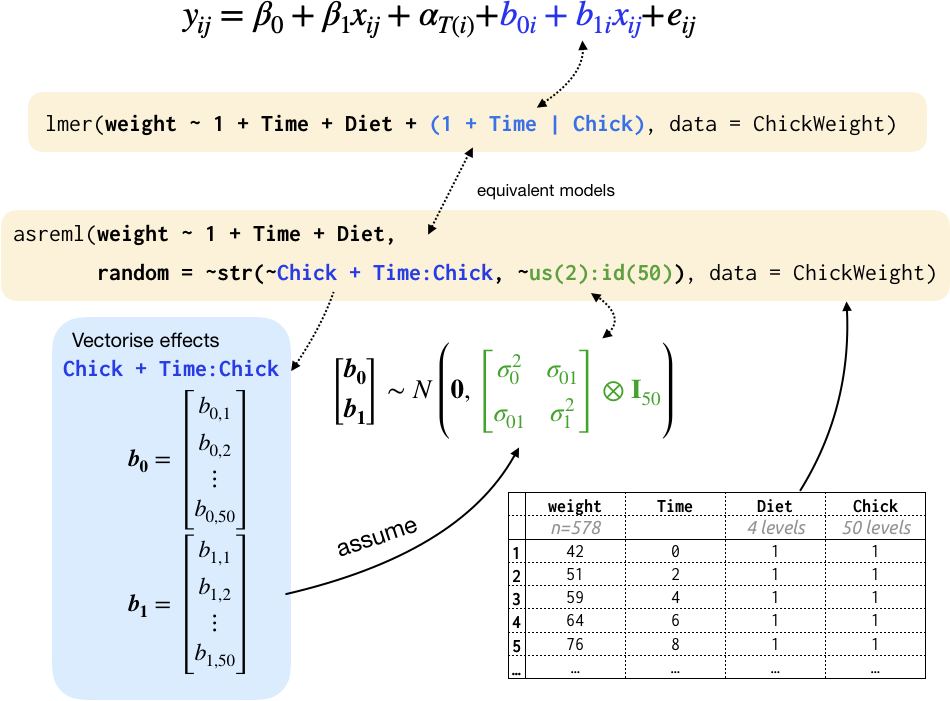
\includegraphics[width=0.9\linewidth,fbox]{images/symbolic_lmm} \caption{This figure shows a longtiduinal analysis of the chicken data (see Section \ref{chick}). The index form of the model equation shows direct resemblance for symbolic model formula in \texttt{lmer} for the fixed and random effects, however, the its covariance form is not as easily inferred. In contrast, the symbolic model formula in \texttt{asreml} show resemblance of the covariance structure specified in the second argument of \texttt{\textasciitilde{}str}, however, the corresponding random effects specified in the first argument of \texttt{\textasciitilde{}str} must be vectorised as show in the above figure. This results in the loss of one-to-one correspondence between effects and symbolic terms for \texttt{asreml}.}\label{fig:symbolic-lmm}
\end{figure}



The model fitted in Figure \ref{fig:symbolic-lmm} is commonly referred to as \emph{random intercept and random slope model} with the diet treatment effect. More specifically, the model
\[y_{ij} = \beta_0 + \beta_1 + \alpha_{T(i)} + b_{0i} + b_{1i}x_{ij} + e_{ij}\]
where \(y_{ij}\) is the weight of the \(i\)-th chicken at time index \(j\); \(x_{ij}\) is the days since birth at time index \(j\) for the \(i\)-th chicken; \(b_{0i}\) and \(b_{1i}\) are random intercept and random time slope effects for the \(i\)-th chicken; \(\beta_0\) and \(\beta_1\) are the overall intercept and slope for time covariate.

\hypertarget{atrial}{%
\subsection{Field Trial: Covariance Structure}\label{atrial}}

\hypertarget{MET}{%
\subsection{Multi-Environmental Trial: Separable Structure}\label{MET}}

\begin{figure}
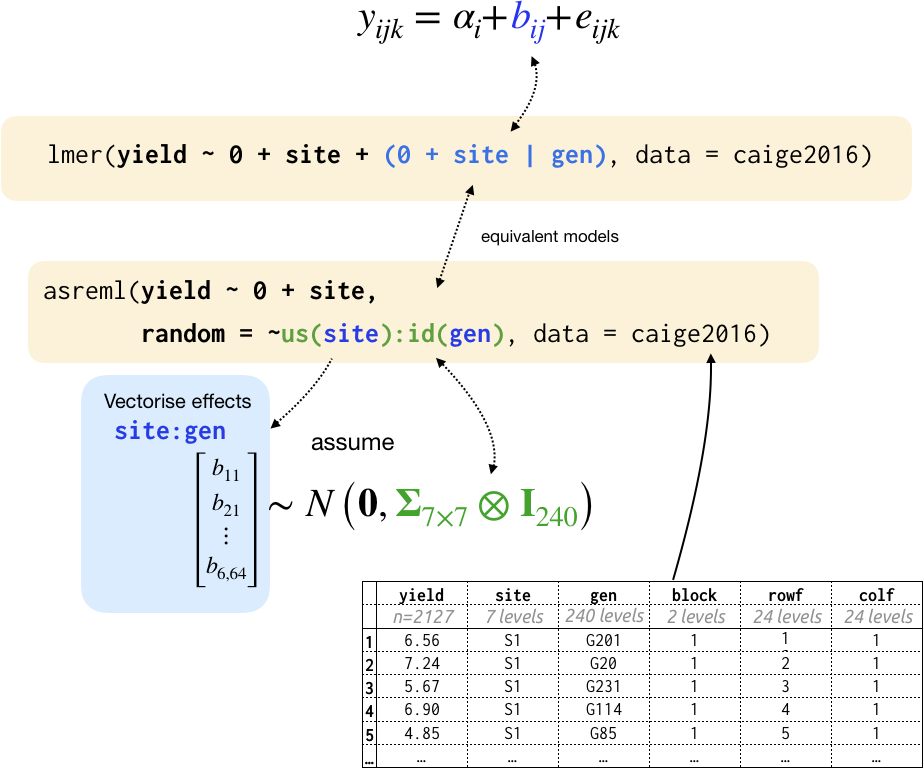
\includegraphics[width=0.9\linewidth,fbox]{images/symbolic_lmm2} \caption{This figure show the fit of a simple mixed mdoel for the analysis of MET data. In modelling the \texttt{county} by \texttt{gen} random effect, the variance structure are specified differently.}\label{fig:symbolic-lmm2}
\end{figure}



\hypertarget{discussion}{%
\section{Discussion}\label{discussion}}

Software packages that fit statistical models have varying input arguments.

Linear (fixed) models are special cases of linear mixed models. As such it is important that the model formula evaluation rules specified in linear models hold true for linear mixed models.

The \texttt{brms} papers make extensive discussion of symbolic model formula and extends on the framework built on \texttt{lme4}. These are noteworthy.

\section*{Acknowledgement}

This paper benefited from twitter conversation with Thomas Lumley. This paper is made using R Markdown \autocite{rmarkdown}. All materials used to produce this paper and its history of changes can be found on github \url{https://github.com/emitanaka/paper-symlmm}.

\printbibliography[title=References]

\end{document}
